\usepackage{graphicx}
\usepackage{array}
\usepackage{longtable}
\usepackage{booktabs}
\usepackage{tabularx}
\usepackage[a4paper,margin=1in]{geometry}

%Engeland,
%Australië, Stockholm, Schotland en Noord-Ierland

\chapter{\IfLanguageName{dutch}{Stand van zaken}{State of the art}}%
\label{ch:stand-van-zaken}

\section{Inleiding}
Internet of Things is over de laatste twintig jaar enorm geëvolueerd, en het gebruik hiervan is wijdverspreid, van boeren in de agrarische sector tot artsen in de gezondheidszorg maken direct en indirect gebruik van IoT. Tegenwoordig worden miljarden van deze apparaten gebruikt door mensen om een verschil te maken in hun respectieve vakgebied. Ook in de gezondheidszorg biedt IoT veel mogelijkheden bij het aanpakken van grote problemen zoals de lange wachttijden in A\&E afdelingen.Diverse landen worden met dit probleem geconfronteerd, zoals Engeland, Australië, Zweden, Schotland en Noord-Ierland \autocite{Friebel2020}. Ook België krijgt hiermee te maken,  volgens een onderzoek uitgevoerd door \TODO Testaankoop wordt geconcludeerd dat Belgische ziekenhuizen wachttijdsproblemen ondervinden, maar dat deze variëren tussen ziekenhuizen. Deze langdurige wachttijden zorgen ervoor dat patiënten in sommige gevallen buitensporige wachttijden ervaren, in enkele gevallen moeten patiënten zelf over de twaalf-uur wachten voor behandelingen. Deze overmatige wachttijden hebben serieuze implicaties en kan in sommige gevallen leiden tot het overlijden van patiënten. Het gebruik van IoT devices biedt hiervoor een mogelijke oplossing om de langdurige wachttijden te verkorten door gebruik te maken van gegevensverzameling en automatisering. Dit hoofdstuk verkent de literatuur om een beter begrip te krijgen over IoT, de werking ervan en hoe het kan gebruikt worden om wachttijden te verminderen. Het hoofdstuk begint met een overzicht over IoT, het ontstaan en de betekenis ervan besproken worden. Verder worden de verschillende componenten van IoT behandeld en in detail wordt uitgewerkt. Vervolgens wordt IoT in de gezondheidszorg besproken waarbij de huidige implementaties hiervan volgens de literatuur worden opgesomd. Hierna komen de voor- en nadelen van IoT in de gezondheidszorg aan bod, gevolgd door een analyse van de beveiligings- en ethische kwesties. Hierop volgt een sectie over de wachttijden in A\&E-afdelingen en de impact hiervan op de zorgkwaliteit. Tot slot wordt besproken hoe IoT kan bijdragen aan het verminderen van de wachttijden met enkele voorbeelden van implementaties uit de literatuur.

\section{Overzicht Internet of Things}
De term \textit{Internet of Things} is ontstaan in 1999, toen Kevin Ashton, een Britse technologiepionier, verschillende objecten probeerde te verbinden met het internet door gebruik te maken van RFID-tags \autocite{Bassi2013, Rejeb2023}. Het concept Internet of Things verwijst naar een netwerk waarin fysieke objecten ('things') via het internet met elkaar communiceren. Deze objecten zijn uitgerust met sensoren en actuatoren om gegevens te kunnen verzamelen, verwerken en delen, waardoor ze slim en interactief worden \autocite{Elksasy2023}. Het concept wordt uiteindelijk beschouwd als een manier waarop verschillende objecten hun aanwezigheid behouden om een samenhangend geheel te vormen voor iedereen, overal, op ieder moment, met ieder medium en ieder netwerk, zoals geïllustreerd in Figuur \ref{fig:Figuur9}. 

\begin{figure}[h]
    \centering
    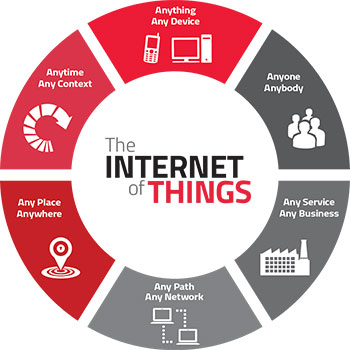
\includegraphics[width=0.4\textwidth]{img/bp/iot-concept.jpg}
    \caption{Internet of Things Networking}
    \label{fig:Figuur9}
    \textit{Source: \autocite{Dauwed2018}}
\end{figure}

Dankzij de voortdurende innovaties in de technologie hebben de laatste twee decennia een grote invloed gehad op de snelle vooruitgang van IoT. \autocite{Almutairi2024}. Hierdoor is het aantal aangesloten IoT devices sterk gestegen, met 7.74 miljard in 2019, 10.7 miljard in 2021 \autocite{Dawod2022} en tot 75 miljard in 2025 \autocite{Khan2019}. Sensoren, camera's en gelijkaardige apparaten worden al “geïntegreerd” in “woningen” en “voertuigen” \autocite{Dawod2022} en geïmplementeerd over verschillende sectoren zoals de “gezondheidszorg, landbouw, productie transport, milieu en nutsbedrijven \autocite{Naresh2020, Almutairi2024}. De implementatie van miljarden \autocite{Dawod2022} IoT devices over verschillende sectoren geeft een duidelijke representatie van de veranderingen die IoT zal brengen in de manier waarop men leeft, werkt en omgaat met de omgeving \autocite{Almutairi2024}. Dit deel heeft verschillende aspecten van IoT behandeld zoals de oorsprong, het concept en het gebruik. Het volgende deel zal dieper ingaan op de hardwarecomponenten om een beter begrip te verkrijgen in de werking van IoT.

%Deze technologie maakt het mogelijk om IoT in te zetten in verschillende sectoren, zoals transport, slimme steden, nutsbedrijven, milieu, gezondheidszorg en veiligheid. Volgens \autocite{Naresh2020} zal dit leiden tot 75 miljard verbonden IoT-devices in 2025 \autocite{Khan2019}. Dit benadrukt het belang van IoT als een technologie en het gebruik hiervan in diverse sectoren. Dit deel heeft verschillende aspecten van IoT behandeld zoals de oorsprong, het concept en het gebruik. Het volgende deel zal dieper ingaan op de hardwarecomponenten om een beter begrip te verkrijgen in de werking van IoT.

%De afgelopen twee decennia hebben een grote invloed gehad op de snelle vooruitgang van IoT \autocite{Almutairi2024}, hierdoor is het aantal aangesloten IoT devices sterk gestegen, met 7.74 miljard in 2019, 10.7 miljard in 2021 \autocite{Dawod2022} en 25.44 miljard tegen 2030 \autocite{Dawod2022}. Sensoren, camera's en gelijkaardige apparaten worden al “geïntegreerd” in “woningen” en “voertuigen” \autocite{Dawod2022} en geïmplementeerd over verschillende sectoren zoals de “gezondheidszorg, landbouw, productie” en slimme steden \autocite{Almutairi2024}.


%Zoals eerder aangetoond beschikt IoT over verschillende componenten die ervoor zorgen dat deze gegevens kan detecteren en verwerken. In het volgende deel worden deze componenten zorgvuldig geanalyseerd. 

\subsection{IoT hardware componenten} 
De IoT-omgeving bevat verschillende belangrijke componenten zoals sensoren, actuatoren, microprocessors, en communicatie protocollen. Deze componenten zorgen ervoor dat objecten slim worden en in staat zijn om met elkaar te communiceren \autocite{Abraham2023, Gharde2024}. In de volgende secties zullen de componenten in detail worden behandeld om een volledig begrip in de werking van IoT te krijgen. De eerste component dat geanalyseerd zal worden zijn de sensoren.

\subsubsection{Sensors}
Sensoren zijn een van de belangrijkste componenten in een IoT-structuur. De functie hiervan is het verzamelen van gegevens in een bepaalde omgeving \autocite{Abraham2023, Moyer2019}. Meer specifiek detecteren de sensoren elke “fysieke of chemische” verandering. Deze gegevens worden vervolgens verwerkt door de applicatie of device om slimme beslissingen te nemen en acties te automatiseren \autocite{Sehrawat2019}. Om een IoT-systeem compleet te maken, worden sensoren gebruikt in samenwerking met actuatoren. Deze worden in de volgende sectie besproken. Zie tabel \ref{tab:sensors} voor een weergave van een aantal IoT sensoren. Deze sensoren worden verder onderverdeeld in verschillende sub types zoals aangetoond door tabel \ref{tab:sensor_subtypes}.

\begin{table}[h]
    \raggedright
    \renewcommand{\arraystretch}{1.3}
    \small
    \caption{Sensor types en het gebruik ervan \autocite{Moyer2019, Sehrawat2019, Kumar2024, Balogun2017, Meenakshi2020, Tresanchez2018, Shanmugavalli2023, Gala2020, Gade2013, Chidurala2021, Karunarathne2018, Srinivasan2022}}
    \begin{tabular}{|c|m{4cm}|m{10cm}|}
        \hline
        \textbf{S/N} & \textbf{Sensor devices} & \textbf{Description} \\
        \hline
        1. & Motion sensor & Een bewegingsdetector is een IoT-device dat gebruikt wordt voor het detecteren van fysieke en dynamische bewegingen. Motion sensing kan ingezet worden om bijvoorbeeld een eigendom te beschermen door potentiële indringers te detecteren. In een onderzoek uitgevoerd door \autocite{Tiong2019} wordt motion sensing gebruikt als IoT-based Home Security System voor het detecteren van indringers. \\
        \hline
        2. & Pressure sensor & Een druksensor worden in IoT-systemen gebruikt om kracht en drukte te meten en detecteren. Deze sensor kan worden gebruikt om de aanwezigheid van gebruikers te monitoren op stoelen en bedden wat real-time informatie biedt\\
        \hline
        3. & Optical proximity sensor & Wordt gebruikt voor het detecteren van objecten door gebruik te maken van licht zonder fysieke contact. \\
        \hline
        4. & Wireless Communication & Is een belangrijk aspect van IoT, deze zorgt ervoor dat devices met elkaar kunnen communiceren door data te delen en verzenden. \\
        \hline
        5. & Thermal camera & Thermische camera's zijn sensoren die gebruikt worden om infrarode radiatie te detecteren van objecten met een temperatuur hoger dan nul graden. Deze sensoren kunnen gebruikt worden voor het monitoren van niet-intusieve bezetting \\
        \hline
        %4. & Magnetometers & Een magnetometer wordt gebruikt om magnetische velden te detecteren. In een studie uitgevoerd door \autocite{Hutagalung2021} worden magnetometers gebruikt in smart parkings. Auto's worden in de parkeerruimte gedetecteerd om te bepalen of een parkeerplaats vrij is of niet. \\
        6. & Proximity sensors & Proximity sensoren worden meestal gebruikt in de industriële en agrarische sector. Deze sensoren maakt gebruik van elektromagnetische velden om te detecteren of een object dichtstbij is. \\
        \hline
        7. & Image sensors & Beeldsensoren geven de omgeving weer door gebruik te maken van fotodiodes. Deze diodes worden gebruikt om licht in een bepaald gebied te detecteren. Beeldsensoren worden toegepast in verschillende systemen en sectoren, ze worden gebruikt in medische beeldsystemen, in digitale camera's, in nachtzichtapparatuur en nog veel meer. Verder worden deze sensoren ook gebruikt in winkels, bijvoorbeeld om de klanten te monitoren. \\
        \hline
    \end{tabular}
    \label{tab:sensors}
\end{table}


\begin{table}[h]
    \raggedright
    \renewcommand{\arraystretch}{1.3}
    \tiny
    \caption{Sensor types en hun subtypes met uitleg \autocite{Yadav2020, Sasi2021, Chawuthai2018, Wei2024, Kleeman2018, Doubek2016, Palanisamy2021, Halvorsen2009, Ghemari2023, Lattanzi2023, Hutagalung2021, Wu2023, Hoberg2011, Lo2013, Braun2015, Vukonic2022, Sarkar2013, BlancoFilgueira2016, RadhaKrishna2021, Mehta2015, Sundar2015, Wu2005, Bieszczad2011, Chen1994, Pop2009, Ajmera2018, Javed2017, Jacobs2009, Preradovic2009, Mockler2010, Spachos2020}}
    \begin{tabular}{|c|m{3cm}|m{3.5cm}|m{7.5cm}|}
        \hline
        \textbf{S/N} & \textbf{Sensor Type} & \textbf{Sub Type} & \textbf{Description} \\
        \hline
        1. & Motion sensor & Passive Infrared (PIR) sensors & Detecteert beweging door veranderingen te waarnemen in infraroodstraling \\
        & & Microwave & Deze sensor zendt microgolven uit, de reflectie van deze golven wordt geanalyseerd om beweging te detecteren. \\
        & & Ultrasonic & Zend en ontvangt geluidsgolven boven de 20 kHz om beweging te detecteren, samen met de afstand tussen objecten. \\
        \hline
        2. & Pressure sensor & Force-Sensitive Resistors & Is een low-cost pressure sensor waarbij de weerstand verandert wanneer kracht gedetecteerd word.\\ & & Strain Gauge Pressure Sensors & Meet drukte door de deformatie van een materiaal te detecteren. \\
        \hline
        3. & Optical proximity sensors & Infrared break beam sensor & Een infrarood emitter en een receiver worden tegenover elkaar geplaatst waardoor er een infrarood licht onstaat. Wanneer een persoon door het licht gaat wordt deze onderbroken waardoor er een detectie geactiveerd wordt.  \\ & &  Diffuse Reflective Optical Sensor & Wordt gebruikt voor objectdetectie en nabijdetectie. Deze sensoren zenden licht uit en meten de gereflecteerde licht van objecten waardoor ze deze kunnen detecteren.\\
        \hline
        4. & Wireless communication protocol & BLE (Bluetooth Low Energy) beacon & Zijn wireless zenders die unieke identifiers uitzenden. \\
        & & Radio Frequency Identification (RFID) & Bestaat uit een tag, reader en middleware software. Maakt gebruik van radio golven om data draadloos te verzenden. \\
        \hline
        5. & Thermal camera & Uncooled thermal camera & Een device voor het detecteren van infrarood radiatie zonder de nood voor een cooling systeem. \\ & & Cooled thermal camera & detecteren infrarode radiatie met hoge snelheid en gevoeligheid door de sensoren naar cryogenische temperaturen te laten dalen. \\
       % 4. & Magnetometers & Fluxgate & Gebruikt voor het detecteren van magnetische velden. \\
       % & & Hall-effect & Detecteren trillingen in gebouwen, worden ook in parkings gebruikt voor het detecteren van de aanwezigheid van voertuigen . \\
       % & & SQUID (Superconducting Quantum Interference Device) & Zeer gevoelige sensor voor zeer zwakke magnetische velden.\\
        \hline
        6. & Proximity sensors & Inductief & Detecteert “geleidende en niet-geleidende materialen” door middel van een elektromagnetische veld  \\
        & & Capacitief & Maakt gebruik van zwakke elektrische velden om “geleidende en niet-geleidende materialen” te detecteren. \\
        & & Ultrasoon &  Wordt gebruik om proximity en afstand te meten door middel van een “hoog-frequentie geluidsgolf”.  \\
        \hline
        7. & Image sensors & Linear image sensor & legt lijn voor lijn afbeeldingen vast door waardoor real-time tracking van stoelbezetting mogelijk is. Kan in de gezondheidszorg gebruikt worden om de bezetting van wachtruimtes en patiëntenflow te monitoren.    \\
        & & Infrared Image Sensors & Detecteert infrarood radiatie en converteert het naar een beeld.\\
        \hline
    \end{tabular}
    \label{tab:sensor_subtypes}
\end{table}


\subsubsection{Actuatoren}
Actuatoren zijn componenten die in staat zijn om het “fysieke wereld” te beïnvloeden op basis van de verzamelde gegevens \autocite{Moyer2019}. Actuatoren werken in samenwerking met sensoren om een compleet IoT-systeem te creëren dat bewaking, controle, logistiek en voorspelling mogelijk maakt in verschillende gebieden zoals landbouw en milieubeheer \autocite{Talavera2017}. In de volgende sectie wordt het IoT-systeem verder toegelicht door de rol van de microprocessoren te introduceren.

\subsubsection{Microprocessors}
Microprocessoren spelen een essentiële rol in IoT-systemen. Deze fungeren als de centrale eenheid in een IoT-device en zijn verantwoordelijk voor het verwerken van sensorgegevens, uitvoeren van berekeningen en het besturen van actuatoren \autocite{Abraham2023, James2021}. In de volgende sectie worden de communicatieprotocollen besproken, die een essentiële onderdeel vormen van IoT-systemen.

\subsubsection{Communicatie protocollen}
Communicatieprotocollen zijn belangrijke onderdelen bij het faciliteren van communicatie tussen twee slimme apparaten. Wat betreft IoT werden er diverse communicatieprotocollen ontwikkeld zoals HTTP, MQTT en XMPP. Het kiezen van een protocol is echter uitdagend door het verschil in energie-efficiëntie, veiligheid en kwaliteit van de dienstverlening. Hierdoor wordt een protocol gekozen op basis van het IoT-systeem \autocite{Anitha2022, Jeddou2020}. Na het verkennen van componenten is het belangrijk om te begrijpen hoe deze technologieën toegepast worden in de gezondheidszorg. In het volgende hoofdstuk wordt specifiek gekeken naar IoT in de gezondheidszorg, samen met de huidige implementaties hiervan in ziekenhuizen. 


\section{Internet of Things gezondheidszorg}
De gezondheidszorg is een cruciaal onderdeel van ons leven en de geleidelijk ouder wordende bevolking samen met verschillende chronische ziektes plaatsen een significante druk hierop. IoT heeft in deze context enorm veel interesse gewekt dankzij de mogelijkheden om de druk op de gezondheidszorg te verlichten \autocite{Baker2017}. Volgens een onderzoek uitgevoerd door \autocite{Shiny2023} kunnen IoT-devices ingezet worden door gezondheidswerkers om gegevens te verzamelen over de fysieke en mentale condities van patiënten om deze beter te begrijpen en voorspellen. Verder vermeldt het onderzoek dat IoT devices kunnen helpen bij vroegtijdige opsporingen van ziektes en het bieden van meer accurate diagnose en behandeling. Volgens een onderzoek uitgevoerd door \autocite{Li2024} is de gezondheidszorg de sector die het meest zal profiteren van de groei van IoT. Verder vermeldt \autocite{Tavakoli2017} het gebruik van IoT als één van de belangrijkste “technologische methoden” om de prestaties van de gezondheidszorg te verhogen. IoT kan op verschillende manieren geïmplementeerd worden om aan specifieke noden te voldoen zoals aangetoond door figuur \ref{fig:Figuur10}. Om een betere inzicht te geven aan deze toepassingen biedt de volgende sectie een overzicht van diverse implementaties van IoT in de gezondheidszorg.

\begin{figure}[h]
    \centering
    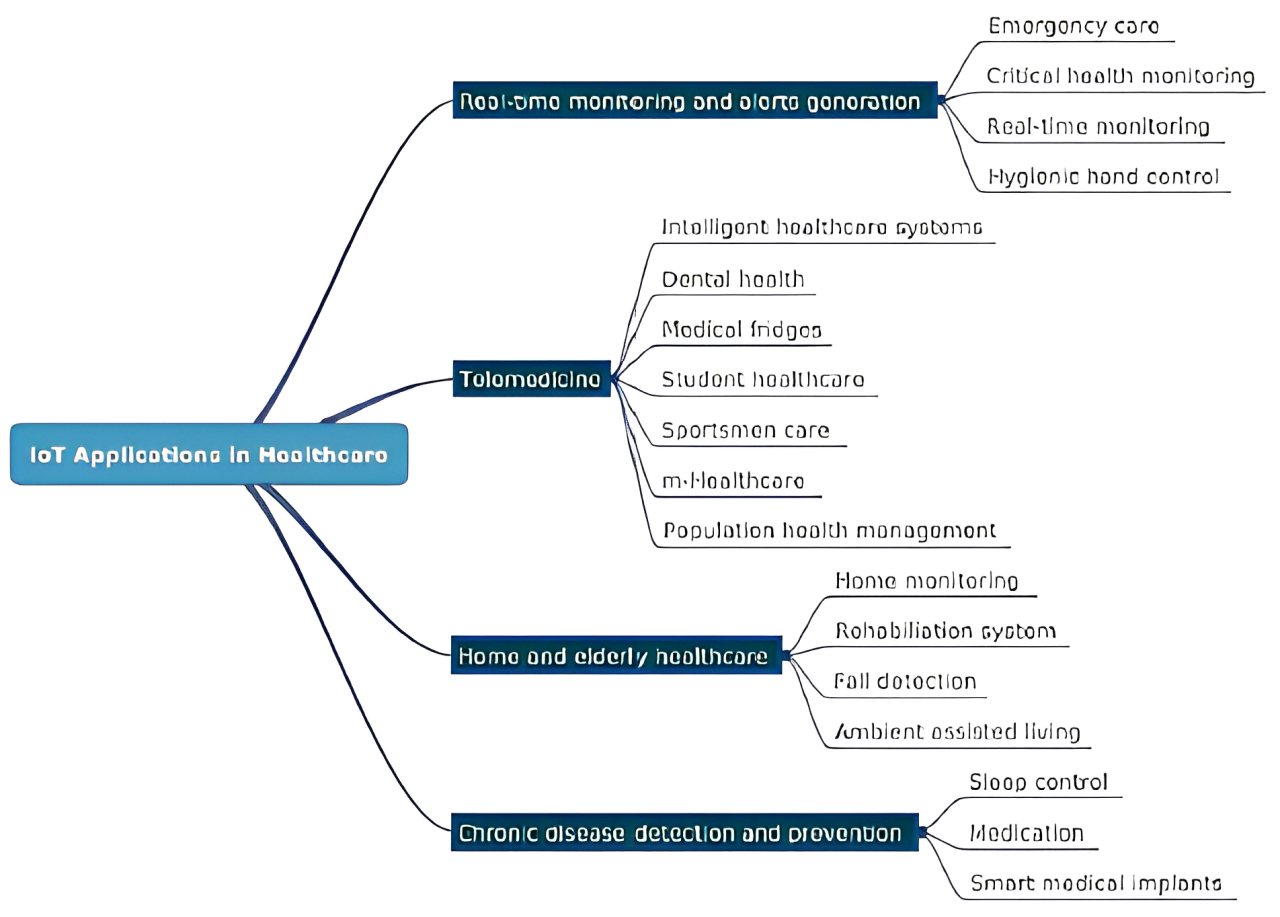
\includegraphics[width=0.75\textwidth]{img/bp/iot-healthcare (1).png}
    \caption{Indeling van IoT-toepassingen in de gezondheidszorg}
    \label{fig:Figuur10}
    \textit{Source: \autocite{Naresh2020}}
\end{figure}

Volgens een recente studie uitgevoerd door \autocite{Singh2023} is het perfect mogelijk om IoT te implementeren in de gezondheidszorg. Echter concludeert het onderzoek dat IoT een gunstige invloed heeft en dit ondanks de beperkingen in “energie, processing en opslag”. Verder benadrukt de studie dat IoT een “veelbelovende technologie” is bij het besparen van tijd en moeite voor het medische personeel. 

\subsection{Huidige implementaties van IoT in de gezondheidszorg}
Een overzicht van implementaties van IoT in het gezondheidszorg: zie figuur \ref{tab:IoT_healthcare}

\begin{table}[h]
    \centering
    \tiny
    \caption{IoT-implementaties in gezondheidszorgstudies \autocite{Mieronkoski2017, Uddin2019, ElZouka2021, Patan2020}}
    \begin{tabularx}{\textwidth}{|p{2cm}|p{1.5cm}|p{3.5cm}|p{3.5cm}|X|}
        \hline
        \textbf{Author and Year} & \textbf{Country} & \textbf{Objectives} & \textbf{IoT Applications} & \textbf{Conclusion} \\
        \hline
        Riitta Mieronkoski  
        & Finland  
        & Voorstellen van IoT aan verpleegkundigen door de stand van zaken over IoT te onderzoeken die betrekking heeft op verpleegkundige zorg in ziekenhuizen.          
        & IoT-innovaties zijn geïdentificeerd in vier verpleegactiviteiten: "comprehensive assessment, periodical clinical reassessment, activities of daily living en care management".  
        & IoT biedt innovaties in verpleegkundige zorg, maar deze innovaties bevinden zich nog in de beginfase. \\  
        \hline
        Md. Zia Uddin  
        & Norway  
        & Ontwikkelen van een systeem dat menselijke activiteiten kan voorspellen door gebruik te maken van wearable healthcare sensors en een Recurrent Neural Network (RNN) op een edge-device.  
        & Verschillende wearable sensoren (ECG, magnetometer, accelerometer en gyroscoop) worden gebruikt voor het monitoren van menselijke activiteiten.  
        & Het gebruik van RNN samen met wearable sensoren op een edge-apparaat vormt een effectief systeem voor het voorspellen van menselijke activiteiten. \\  
        \hline
        Hesham A. El Zouka, Mustafa M. Hosni  
        & Egypt  
        & Het doel is om een slim healthcare-model te ontwikkelen dat automatisch de prioriteit van patiënten bepaalt op basis van gegevens uit sensoren.  
        & IoT-apparaten, WMSN en RFID monitoren patiëntgegevens zoals temperatuur, hartslag en bloeddruk.  
        & Het integreren van fuzzy, AI en IoT biedt real-time monitoring en veilige communicatie. Dit systeem zorgt voor betere patiëntenzorg. \\  
        \hline
        Rizwan Patan, G S Pradeep Ghantasala, Ramesh Sekaran, Deepak Gupta, Manikandan Ramachandran  
        & India  
        & GFB-CNN vermindert communicatie-overhead en responstijd en verhoogt de nauwkeurigheid van medische data-analyse.  
        & IoT wordt toegepast in smart healthcare. IoT-sensoren verzamelen en verzenden medische data voor real-time analyse.  
        & De GFB-CNN-methode verbetert de analyse van medische data door de analysetijd te verkorten. \\  
        \hline
    \end{tabularx}
    \label{tab:IoT_healthcare}
\end{table}


%\section{Voordelen en uitdagingen van IoT in de gezondheidszorg}
%In dit deel worden de voor- en nadelen van IoT in de gezondheidszorg opgenomen volgens de literatuur. Hierbij wordt er rekening gehouden met hoe IoT de gezondheidszorg beïnvloedt en hoe deze de gezondheidszorg heeft getransformeerd. In de volgende secties worden eerst de voordelen besproken gevolgd door de uitdagingen die hierbij horen.


%\subsection{Voordelen}
%Door zorgverleners in staat te stellen om IoT te benutten is het mogelijk om “patiëntresultaten te verbeteren, het gebruik van middelen te optimaliseren, de operationele efficiëntie te verhogen, en patiënten in staat stellen actief deel te nemen aan hun eigen zorg wordt mogelijk gemaakt” \autocite{Inzole2024}. Er zijn een onbeperkt aantal mogelijkheden om de gezondheidszorg te verbeteren door gebruik te maken van IoT, hier zijn enkele belangrijke verbeteringen die IoT brengt \autocite{Inzole2024, Abdulmalek2022}. 

%\begin{itemize}
%    \item Beter behandeling van patiënten
%    \item Vroeg opsporen van ziektes
%    \item Kost van behandeling verminderen
%    \item Beter monitoren en beheren van patiënten
%    \item Verhoogd efficiëntie en verbeterde middelen gebruik
%\end{itemize}

%Ondanks de vele voordelen introduceert IoT ook een aantal uitdagingen, deze worden in het volgende sectie besproken. 

%\subsection{Uitdagingen}
%Hoewel IoT belangrijke voordelen levert aan de gezondheidszorg, brengt IoT nog steeds veel problemen met zich mee zoals aangetoond door figuur \ref{fig:Figuur13}. Het analyseren van deze problemen is essentieel voordat IoT geïmplementeerd kan worden om mitigerende strategieën te bedenken zodat IoT op een verantwoordelijke manier kan uitgerold worden. Hier zijn enkele nadelen van IoT in het gezondheidszorgomgeving \autocite{Inzole2024, Abdulmalek2022}.


%\begin{itemize}
%    \item Security
%    \item Privacy
%    \item Interoperabiliteit
%    \item Naleving van regelgeving
%    \item Ethische consideraties
%\end{itemize}

%\begin{figure}[h]
%    \centering
%    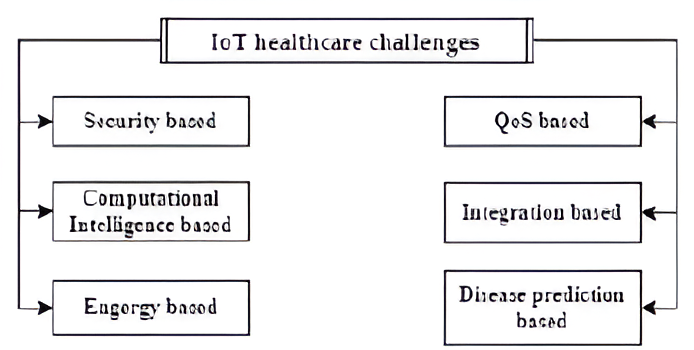
\includegraphics[width=0.60\textwidth]{img/bp/iot-challenges.png}
%    \caption{Nadelen van IoT in het gezondheidszorg}
%    \label{fig:Figuur13}
%    \textit{Source: \autocite{Abdulmalek2022}}
%\end{figure}


%In het volgende deel worden de uitdagingen verder toegelicht, met een specifiek focus op de beveiligings- en ethische kwesties.


%\section{Beveiliging en ethische kwesties van IoT in de gezondheidszorg}
%Met het naadloze integratie van IoT in ziekenhuizen worden patiënten gegevens zorgvuldig verzameld en geanalyseerd waardoor iedere patiënt dezelfde medische diensten kan verwachten. Het gebruik van IoT zorgt ervoor dat patiënten zich niet meer constant hoeven te verplaatsen tussen het ziekenhuis en woonplaats waardoor het niet alleen de sociale lasten maar ook het financiële druk verlaagd \autocite{Chang2019}. Echter, produceren en verzamelen medische instellingen enorme hoeveelheid data (big data) zoals medische dossiers, ziekenhuisdossiers, medische- en biomedische onderzoeksdossiers \autocite{Mirza2022}. Hierbij ontstaan er verschillende beveiligings- en privacy risico's voor patiëntgegevens en vertrouwelijkheid. Deze hebben ernstige gevolgen voor patiënten maar ook voor het vertrouwen in biomedische onderzoeken \autocite{Pandey2018, Juengst2014}. In de volgende sectie worden de beveiligings- en ethische uitdagingen verder in detail uitgewerkt.

%\subsection{Beveiliging} 
%Security problemen zijn een reden voor bezorgdheden vooral door het “enorme snelheid en volumes” waarin medische data wordt gegenereerd. Security wordt gedefinieerd als de “confidentiality, integrity en availability” van het verzamelde data die door het systeem worden verstuurd \autocite{Mittelstadt2017}. Hierbij ontstaan er verschillende security risico's en dit zoals Spoofing, Injection of false signals, Replay attacks, Eavesdropping \autocite{Mirza2022}. Deze risico's ontstaan door “inadequate privacy policies, menselijke fouten, verouderde of onveilige medische apparaten en technologische incompatibiliteit waardoor patiëntengegevens kwetsbaar worden voor misbruik \autocite{Popescul2018}. Ernstige gevolgen kunnen hieruit volgen, waaronder het verlies van mensenlevens, hierdoor wordt security beschouwt als van primordiaal belang \autocite{Ali2024}. Ondanks de uitdagingen dat security met zich meebrengt in IoT is dit niet de enige uitdaging, in het volgende sectie worden de ethische uitdagingen verder besproken.

%\subsubsection{Ethiek}
%Sociale gedrag normen in IoT omvatten beide ethiek en moraal. Ethiek wordt gedefinieerd als hetgeen dat moreel goed of slecht is, en wat fout of juist is, terwijl moraal gedefinieerd wordt als een standaard van normen en regels voor goed gedrag in de samenleving. Ethische gedrag vereist dat men zich houdt aan de volgende richtlijnen \autocite{AboBakr2017, Xhemajli2021}:

%\begin{itemize}
%    \item Privacy van gegevens
%    \item Toegang tot gegevens
%    \item Integriteit van gegevens
%\end{itemize}

%Ethische problemen volgens \autocite{Zakerabasali2022} zijn een van de meest belangrijke en complexe probleem binnen IoT, waardoor het mitigeren hiervan van hoge prioriteit is tijdens de implementatiefase. Figuur \ref{fig:Figuur14} toont de belangrijkste ethische problemen in IoT. 


%\begin{figure}[h]
%    \centering
%    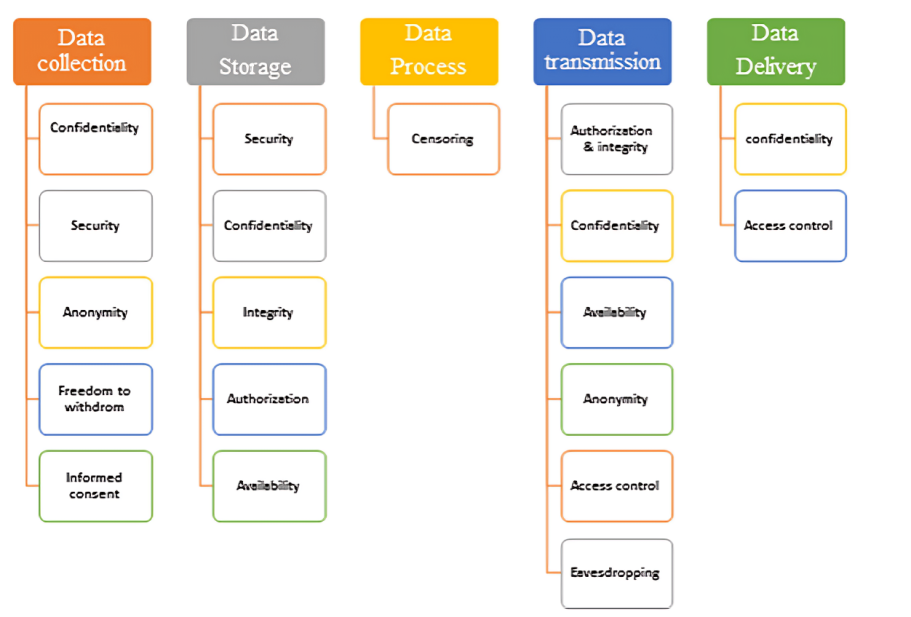
\includegraphics[width=1\textwidth]{img/bp/iot-ethical-issues (1).png}
%    \caption{Ethische kwesties gebaseerd op implementatiefasen van een IoT-systeem.}
%   \label{fig:Figuur14}
%    \textit{Source: \autocite{Zakerabasali2022}}
%\end{figure}

%In het volgende sectie wordt er bekeken naar belangrijke mitigatie strategieën tegen beveiliging en ethische risico's.

%\subsubsection{Mitigatie strategieën}
%De security risico's in IoT kunnen op verschillende manieren gemitigeerd worden zoals het implementeren van “technische maatregelen, policy frameworks en gebruikers educatie”. Deze omvatten de volgende strategieën \autocite{Iwuanyanwu2023}: 

%\begin{itemize}
%    \item Technische maatregelen:“Encryption and Secure Communication, Robust Authentication Mechanism, Software and Firmware Updates en Intrusion Detection Systems (IDS)”
%    \item policy frameworks: “Compliance with Industry Standards and Regulations, Legal Frameworks for IoT Security“
%    \item gebruikers educatie: “Training Programs for End-Users, Promoting Secure IoT Practices”
%\end{itemize}

%De ethische risico's kunnen op diverse manieren worden aangepakt, maar het idee is dat één enkele mitigatie strategie niet genoeg kan zijn om meerdere ethische problemen te behandelen. Daarom wordt er voorgesteld om verschillende strategieën te combineren zoals: 

%\begin{itemize}
%    \item “ethisch gedrag bij het programmeren”
%    \item “whitebox-algoritmen”
%    \item “blackbox-validatie”
%    \item “algoritmische sociale contracten”
%    \item “omhullende IoT-systemen”
%    \item “richtlijnen en ethische code voor IoT-ontwikkelaars”
%%\end{itemize}

%Het combineren van deze strategieën kan ervoor zorgen dat alle aspecten van verschillende ethische risico's behandeld worden \autocite{Loke2019}. Na het bespreken van de beveiliging en ethische kwesties van IoT wordt de focus gelegd op de kern van het onderzoek. In de volgende secties zullen verschillende onderdelen besproken worden die hiermee verband houden. Eerst zullen de wachttijden op de A\&E-afdelingen behandeld worden. Vervolgens zal de impact hiervan op het zorgkwaliteit uitgebreid worden besproken. Tot slot worden de IoT-devices die deze probleem kunnen verhelpen opgesomd en besproken. 

\section{Wachttijden in A\&E-afdelingen}
De vraag naar spoedeisende hulp is in veel landen gestegen zoals in Engeland,
Australië, Stockholm, Schotland en Noord-Ierland waardoor het steeds moeilijker is om doorlooptijden kort te houden. Verschillende factoren zijn de oorzaak van dit probleem zoals het veroudering van de populatie, complexere ziektes en de toenemende vraag van patiënten voor spoedeisende zorg. Volgens studies uitgevoerd door \autocite{Paling2020, Friebel2020} door is bedbezetting nauw verbonden met hoge wachttijden, zoals aangetoond in Figuur \ref{fig:Figuur11} is er een correlatie tussen de hoge wachttijden en bedbezetting.

\begin{figure}[h]
    \centering
    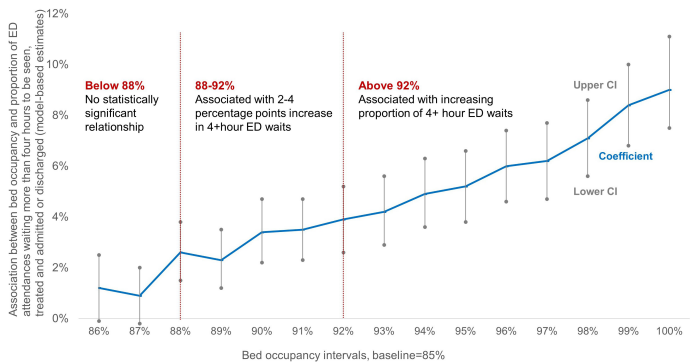
\includegraphics[width=0.80\textwidth]{img/bp/bed-occupancy.png}
    \caption{Plot dat een niet-lineaire relatie toont tussen bedbezettingen intervallen en proportie van patiënten die meer dan vier uur spenderen in de A\&E-afdeling}
    \label{fig:Figuur11}
    \textit{Source: \autocite{Paling2020}}
\end{figure}

Om dit probleem tegen te gaan hebben meerdere landen een wachttijdsstandaard geïmplementeerd om de wachttijden in kaart te brengen en deze gevolgen te verminderen \autocite{Paling2020}. In de Verenigd Koninkrijk bijvoorbeeld is “tijdigheid” een cruciaal aspect in het kwaliteit van spoedeisende hulp, en de wachttijddoelstellingen van de National Health Service zijn hierop gebaseerd voor A\&E afdelingen in het hele Verenigd Koninkrijk. Deze wachttijddoelstellingen eisen dat 98 percent van de A\&E patiënten binnen de vier uur van de aankomst worden ontslagen, overgeplaatst of opgenomen worden in een ziekenhuis \autocite{Mayhew2008, Izady2012}. 


Echter wordt er aan deze vier-uur standaard nauwelijks voldaan. Volgens een studie uitgevoerd door \autocite{Baker2024} is het percentage van patiënten die langer dan vier uur in de A\&E-afdelingen spenderen tussen 2015 en 2020 sterk toegenomen. Verder toont het onderzoek dat er een nieuw record bereikt is met 50,4\% van patiënten die langer dan vier uur wachten op behandeling in A\&E-afdelingen zoals aangetoond door figuur \ref{fig:Figuur12}. Dit vormt een duidelijke overtreding van de vier-uur norm van de NHS. Deze richtlijn houdt in dat tenminste 95\% van de patiënten binnen vier uur moeten worden opgenomen, overgebracht en ontslagen. \autocite{NationalStatisticsONS2024}.

\begin{figure}[h]
    \centering
    \includegraphics[width=0.80\textwidth]{img/bp/patiënts_over_4_hours.png}
    \caption{Percentage van patiënten die langer dan 4 uur wachten}
    \label{fig:Figuur12}
    \textit{Source: \autocite{Baker2024}}
\end{figure}

% Link volgende stuk
Deze lange wachttijden hebben serieuze gevolgen op de patiëntentevredenheid en zorgkwaliteit zoals besproken in het volgende hoofdstuk.

\subsection{Impact van wachttijden op de zorgkwaliteit}
Volgens verschillende studies hebben langdurige wachttijden negatieve gevolgen voor zowel patiënten als de zorgkwaliteit. Studies uitgevoerd door \autocite{Vainieri2020, QuintonJ.Nottingham2018, Bleustein2014} benadrukken de negatieve impact van de wachttijden op de patiëntentevredenheid. Deze onderzoeken tonen aan dat lange wachttijden een ongunstige invloed op de tevredenheid van patiënten, vooral in het vertrouwen van de zorgverleners en kwaliteit van de zorg. Verder benadrukt een studie uitgevoerd door \autocite{Paling2020} nog ernstigere gevolgen voor patiënten, deze onderzoek heeft een verband gesteld tussen wachttijden in A\&E-afdelingen en een hogere mortaliteit en verergeren van resultaten voor patiënten. Echter, zijn patiënten niet de enige die door de lange wachttijden worden beïnvloed, volgens \autocite{Osborne2015} ervaren duizenden verpleegsters in Engeland moeilijkheden bij het omgaan met de lange A\&E-wachttijden, het artikel vermeldt verder een quote door de toenmalige RCN emergency care association chair, Janet Youd, die aangaf dat 'verpleegsters zijn uitgeput en velen worden ziek door stressgerelateerde aandoeningen'. Onderzoekers hebben onlangs de werkomstandigheden van NHS werknemers onderzocht. De studie toont dat 40\% van alle ziekten bij het personeel te wijten is aan stress. Verder wijst het onderzoek uit dat de “overheersende stressfactor” wordt veroorzaakt door de hoge werkdruk \autocite{Ravalier2020}. \autocite{Vainieri2020} onderlijnt overbevolking als oorzaak van de hoge werkbelasting, en dit in A\&E departementen in diverse westerse landen. Hierbij wordt er verder benadrukt van de ernst van het probleem voor zowel patiënten als zorgverleners. Deze probleem kan door diverse IoT devices verholpen worden. Dit wordt in het volgende sectie verder besproken. 


% \autocite{Vainieri2020} onderlijnt overbevolking als oorzaak van de hoge werkbelasting, en dit in A\&E departementen in diverse westerse landen. Om beter te begrijpen hoe IoT dit probleem kan oplossen, is het noodzakelijk om dieper in te gaan op wat IoT precies inhoudt. Over het algemeen verwijst Internet of things (IoT) naar een model dat verschillende technologieën omvat. Anders gezegd, is het een netwerk van elektronische apparaten die met elkaar of met de cloud communiceren via het internet. De afgelopen twee decennia hebben een grote invloed gehad op de snelle vooruitgang van IoT \autocite{Almutairi2024}, hierdoor is het aantal aangesloten IoT devices sterk gestegen, met 7.74 miljard in 2019, 10.7 miljard in 2021 \autocite{Dawod2022} en 25.44 miljard tegen 2030 \autocite{Dawod2022}. Sensoren, camera's en gelijkaardige apparaten worden al “geïntegreerd” in “woningen” en “voertuigen” \autocite{Dawod2022} en geïmplementeerd over verschillende sectoren zoals de “gezondheidszorg, landbouw, productie” en slimme steden \autocite{Almutairi2024}.

\section{Internet of Things bij het verkorten van wachttijden in het gezondheidszorg}
IoT heeft zich veelbelovend getoond bij het verminderen van wachttijden in de gezondheidszorg en het verbeteren van de patiëntenzorg \autocite{Bhatt2017}. Diverse studies tonen verschillende implementaties van IoT in de gezondheidszorg en in wachtruimtes \ref{wachtruimte} met als doel om wachttijden te verminderen, zoals aangetoond in tabel \ref{tab:IoT_waiting_time_reduction_healthcare} 

\begin{table}[h]
    \centering
    \tiny
    \caption{Studies: IoT implementaties om wachttijden te verminderen in gezondheidszorg \autocite{Sierra2017, McNabb2018, Alabduljabbar2022, Bhatt2017, Fischer2020, Chandy2019}}
    \begin{tabularx}{\textwidth}{|p{1.7cm}|p{0.9cm}|p{3.5cm}|p{3.5cm}|X|}
        \hline
        \textbf{Author and Year} & \textbf{Country} & \textbf{Objectives} & \textbf{IoT Applications} & \textbf{Conclusion} \\
        \hline
        Pedro Santiago Sierra, Jeyson Bolivar Siculaba, Giovanny Mauricio Tarazona   
        & Colombia 
        & Ontwikkelen van een mobile applicatie waarmee gebruikers instaat zijn om de verschillende wachttijden van diverse zorgpunten te raadplegen. 
        & IoT-gebaseerde sensoren worden op de zorgpunten geïmplementeerd om real-time data te verzamelen 
        & De ontwikkeling en simulatie tonen aan dat de applicatie de gebruiker in staat stelt om zorgpunten te selecteren met de kortste wachttijden. \\
        \hline
        Tim McNabb, Trina Myers*, Kristin Wicking, Lei Lei en Wei Xiang 
        & Australia 
        & Optimaliseren van high-value clinical spaces in de gezondheidszorg door gebruik te maken van IoT. 
        & Drie types werden gebruikt in de eindfase: “infra-red break-beam”, “photovoltaic infra-red (PIR)” en  “photovoltaic array” 
        & De conclusie toont aan dat PIR-sensoren niet voldoende zijn om bezettingen te detecteren.  \\
        \hline
        Reham Alabduljabbar* 
        & Saudi Arabia 
        & Het doel is om een location-aware mobile-based solution (UrNext) te introduceren en te evalueren om wachttijden te verminderen. 
        & Bluetooth Low-Energy (BLE) technology wordt gebruikt om locatie te bieden in ziekenhuizen 
        & UrNext biedt de mogelijkheid om wachttijden te verminderen door gebruik te maken van BLE-technologieën. \\
        \hline
        Yesha Bhatt, Chintan Bhatt 
        & India 
        & Wachttijden elimineren en ziekenhuis bezoeken verminderen door het implementeren van remote healthcare via IoT.
        & Deze implementatie maakt gebruik van Medical devices met IoT features, Biomedical sensors, Smart devices voor patient-nurse connectivity, 24/7 patient monitoring systems.
        & IoT in de gezondheidszorg is steeds in de ontwikkeling phase, verschillende uitdagingen moeten nog geadresseerd worden maar het heeft de potentieel om de industrie te revolutioneren.   \\
        \hline
        Abraham Chandy
        & India 
        & Wachttijden verminderen en medische beeldvorming verbeteren door automatisatie en optimalisatie.
        & IoT wordt gebruikt in medische beeldvorming en medische apparatuur.
        & IoT-enabled medische beeldvorming kan de efficiëntie van de gezondheidszorg verbeteren, kosten verminderen en diagnoses verbeteren.    \\
        \hline
        Gabriel Souto Fischer,
        Rodrigo da Rosa Righ,
        Gabriel de Oliveira Ramos,
        Cristiano André da Costa,
        Joel J.P.C. Rodrigues
        & Brazil 
        & ElHealth heeft als doel om de toewijzing van de gezondheidszorgprofessional te optimaliseren door gebruik te maken van IoT om wachttijden te verminderen.
        & Occupancy sensors, patiënt monitoring systemen en omgeving sensoren worden gebruikt om ruimte gebruik en behoeften van patiënten bij te houden.
        & De ElHealth maakt gebruik van voorspellingen en dynamische personeel toewijzing om wachttijden te verminderen processen te optimaliseren.    \\
        \hline
    \end{tabularx}
    \label{tab:IoT_waiting_time_reduction_healthcare}
\end{table}

\subsection{Implementaties van IoT in wachtruimtes} \label{wachtruimte}

\begin{table}[h]
    \centering
    \tiny
    \caption{Studies: IoT implementaties om wachttijden te verminderen in gezondheidszorg \autocite{Spoladore2024, Ghazal2015}}
    \begin{tabularx}{\textwidth}{|p{2.5cm}|p{1cm}|p{4cm}|p{4.5cm}|p{3cm}|}
        \hline
        \textbf{Author and Year} & \textbf{Country} & \textbf{Objectives} & \textbf{IoT Applications} & \textbf{Conclusion} \\
        \hline
        Daniele Spoladore, Marta Mondellini, Atieh Mahroo, Irene Alice Margherita Chicchi Giglioli, Stefano De Gaspari, Daniele Di Lernia, Giuseppe Riva, Elena Bellini, Nicoletta Setola, Marco Sacco   
        & Italy 
        & Onderzoeken hoe IoT, AI en Virtual reality een wachtruimte kan transformeren in een smart omgeving. 
        & De Age-IT prototype maakt gebruik van IoT sensoren, AI en virtual reality.
        & Dit systeem biedt een significante stap bij het transformeren van traditionele wachtruimtes in een smart omgeving en het omzetten van wachttijden in diagnostische en therapeutische activiteiten. \\
        \hline
        M. Ghazal, Rania Hamouda, Samr Ali
        & Bahrain 
        & Het doel is om de queue management te verbeteren door de service kwaliteit te verhogen en wachttijden te verminderen
        & Het systeem maakt gebruik van ESP32 om live queue data te versturen.
        & Het systeem werkt zoals weergegeven in de studie.  \\
        \hline
    \end{tabularx}
    \label{tab:IoT_waiting_time_reduction_waitingroom}
\end{table}


\section{Plaatsing strategieën van IoT}
De plaatsing van een IoT device wordt gecategoriseerd worden in twee diverse plaatsing strategieën, de fysieke plaatsing en netwerk plaatsen. In de netwerkplaatsing wordt de focus gelegd op de plaatsing van de IoT-gateways. Aangezien deze buiten de scope van het onderzoek vallen, zijn alleen de fysieke plaatsing en relevante aspecten van belang. Deze worden in de volgende sectie verder toegelicht.

\subsection{Physical placement}
Fysieke plaatsing is de manier waarop een device “strategisch geplaatst” wordt voor een betere netwerk performantie en dekking \autocite{Xia2018}. Zie tabel \ref{tab:placement_strategies} voor een overzicht van diverse fysieke plaatsing strategieën.

\begin{table}[h]
    \centering
    \tiny
    \caption{Physical Placement Strategies for IoT Devices, \autocite{Tinglib2012, Alablani2019, Badiger2022, Chen2023, Krishnachalitha2020, Patil2021, Paul2020}}
    \begin{tabular}{|l|p{4cm}|p{5cm}|p{4cm}|} % Adjusted last column width
        \hline
        \textbf{Strategy} & \textbf{Goal} & \textbf{Approach/Method} & \textbf{Benefits} \\ \hline
        Uniform Random Deployment & Devices worden random verspreid om dekking te hebben over een gebied. Uniform deployment is een gemeenschappelijke strategie voor het uitrollen van IoT devices en sensoren in een wireless netwerk  & Devices worden op een uniforme wijze verspreid over een bepaald gebied. & Makkelijk te implementeren, maar heeft weinig dekking en is minder veerkrachtig tegen aanvallen. \\ \hline
        Grid-Based Deployment & biedt predictive en gestructureerde dekking voor wireless netwerken  & Devices worden uitgerold in een geometrische pattern zoals square grids, triangular grids, or hexagonal grids om voor een uniforme dekking te zorgen. De square grid heeft een hogere performantie in de dekking van gebieden terwijl de andere beter in end-to-end delay zijn. & voorspelbaar en makkelijk te analyseren dekking gebied. \\ \hline
        Cluster-Based Deployment & Heeft als doel om data aggregation te optimaliseren en het verminderen van energie consumptie. & Devices worden gegroepeerd in clusters, een centrale nood worden vervolgens gebruikt voor data aggregation en energy efficiënte solutions. & Verminderd data redundancy en communicatie overhead. \\ \hline
        Mobility-Aware Deployment & De IoT devices worden geplaatst op basis van de beweging pattern van devices of users & Devices worden dynamisch geplaatst volgens voorspelde beweging patterns. & Verminderd de energie consumptie en verbetert de plaatsing efficiëntie \\ \hline
        Fixed Placement & Zorgt ervoor dat de data verzameling consistent en betrouwbaar is. & Devices worden op permanente locaties geïnstalleerd, dit zorgt voor een sterke netwerk performantie en verbruik van middelen. & Betrouwbaar en makkelijk te onderhouden \\ \hline
    \end{tabular}
    \label{tab:placement_strategies}
\end{table}


%\subsection{Network placement}
%In Netwerk plaatsing wordt de focus gelegd op de plaatsing van de IoT gateways, om kosten te verminderen en performantie te verhogen \autocite{Patil2021, Patil2021a}. Zie tabel \ref{tab:network_placement_strategies} voor enkele praktische voor beelden van Netwerk strategieën.

%\begin{table}[h]
%    \tiny
%    \caption{Network Placement Strategies for IoT Gateways, \autocite{Mnguni2019, Patil2021a, Patil2021, Beuchat2019, Kotagi2017, Nezami2020, Matni2020, Dautov2017}}
%    \begin{tabular}{|p{3.5cm}|p{6.5cm}|p{4.5cm}|}
%        \hline
%        \textbf{Strategy} & \textbf{Description} & \textbf{Benefits} \\ \hline
%        Fixed Gateway Placement & Gateways worden strategisch geplaatst om de dekking te maximaliseren en de netwerk performantie te verbeteren. & Betrouwbare kwaliteit van de service en vermindering van de kosten. \\ \hline
%        Distance-Based Optimization & Gateways worden geplaatst door middel van optimalisatietechnieken zoals Euclidische of Manhattan-afstand om energieverbruik en latentie te minimaliseren. & Efficiënter gebruik van netwerkbronnen en minder energieverbruik. \\ \hline
%        Load-Balanced Placement & Gateways worden geplaatst op basis van de verkeersbelasting. Load balancing is essentieel bij het verbeteren van netwerk performantie en vermijden van congesties. & Consequente verbetering in netwerk performantie en vertraging. \\ \hline
%        Dynamic Gateway Placement & Gateways wijzigen hun positie op basis van veranderende netwerkcondities, zoals gebruikersmobiliteit of variërende dataverkeerpatronen. & Verminderen van de kosten en betere QoS in dynamische IoT-omgevingen. \\ \hline
%        Hierarchical Gateway Deployment & Meerdere niveaus van gateways worden gebruikt om de belasting te verminderen en reactietijd te verhogen. De lagere niveaus verwerken lokaal, terwijl de hogere niveaus verantwoordelijk zijn voor het versturen van data naar de cloud. & Efficiëntere data-agregatie en verminderde latentie. \\ \hline
%    \end{tabular}
%    \label{tab:network_placement_strategies}
%\end{table}


%\section{Evaluatie van software voor IoT-implementaties}
%Diverse software worden gebruikt om communicatie, verwerking, analyse mogelijk te maken in IoT-implementaties. Het doel van deze sectie is om verschillende software te identificeren door diverse studies te verkennen. Het volgende tabel \ref{tab:software_literatuurstudie} toont een overzicht van onderzoeken

%\begin{table}[h]
%    \tiny
%    \caption{Overzicht van onderzoeken naar softwaregebruik in IoT-implementaties, \autocite{Vikash2020}, \autocite{Giacobbe2020}}
%    \begin{tabular}{|p{2.5cm}|p{4.7cm}|p{5.7cm}|p{3.5cm}|}
%        \hline
%        \textbf{Author} & \textbf{Software} & \textbf{Application} & \textbf{Key findings} \\ 
%        \hline
%        Vikash, Lalita Mishra, Shirshu Varma & Apache NiFi & Automatiseert datastroom tussen systemen  & NiFi biedt hoog throughput en lage latency, is ideal voor gebruik met IoT \\ 
%        \hline
%        Vikash, Lalita Mishra, Shirshu Varma & Apache Storm & Verwerken van real-time, unbounded datastreams & Neemt de kortste opstarttijd. \\ 
%        \hline
%        Vikash, Lalita Mishra, Shirshu Varma & Apache Apex & Ondersteunt streams en batch processing voor real-time big data applications & Minst bruikbare solution voor IoT, biedt low throughput, hoog response time, en maximum jitter. \\ 
%        \hline
%        Vikash, Lalita Mishra, Shirshu Varma & Spark Streaming & Verwerkt in real-time batch data door de taken te verdelen over clusters & N.V.T. \\ 
%        \hline
%        Vikash, Lalita Mishra, Shirshu Varma & Apache Flink & Real-time verwerking van batch data door master, slave architectuur te gebruiken voor parallel uitvoer van taken& Minst scalable solution.  \\ 
%        \hline
%        Maurizio Giacobbe, Chakib Chaouch, Marco Scarpa, Antonio Puliafito & InfluxDB & Time series data store voor IoT en real-time analyse & Verzamelt tijdstempels, id's en sensorgegevens zoals temperatuur, helderheid, kooldioxide in smart city-platform. \\ 
%        \hline
%        Robert Stackowiak & Microsoft Azure IoT Suite: Azure IoT Hub & Maakt verbinding en beheer van IoT-devices mogelijk. & N.V.T. \\ 
%        \hline
%        Robert Stackowiak & Microsoft Azure IoT Suite: Azure Digital Twins & Maakt gebruk van ruimtelijke intelligentiegrafieken om een virtuele weergave van de fysieke wereld te maken & N.V.T. \\ 
%        \hline
%        Robert Stackowiak & Microsoft Azure IoT Suite: Azure Stream Analytics & Verwerkt hoge volumes streaming data van devices via SQL queries  & N.V.T. \\ 
%        \hline
%        Robert Stackowiak & Microsoft Azure IoT Suite: Azure Time Series Insights & Maakt de analyse en visualisatie van time series data van IoT-devices.   & N.V.T. \\ 
%        \hline
%        Robert Stackowiak & Microsoft Azure IoT Suite: Azure Databricks & Biedt real-time data verwerking, machine learning en autoscalling van IoT  & N.V.T. \\ 
%        \hline
%        Robert Stackowiak & Microsoft Azure IoT Suite: Azure Data Lake Storage & Azure Data Lake Storage Gen2 combineert de kosteneffectiviteit van Azure Blob Storage met verbeterde functies voor het bestandssysteem  & N.V.T. \\ 
%        \hline
%        Robert Stackowiak & Microsoft Azure IoT Suite: Azure HDInsight & Verwerkt en analyseert big data en ondersteunt diverse open-source frameworks& N.V.T. \\ 
%        \hline
%    \end{tabular}
%       \label{tab:software_literatuurstudie}
%\end{table}



%\subsection{Vergelijking: Traditionele versus IoT-gebaseerde wachttijdsreductie}

% De term 'Internet of Things' is ontstaan in 1999, toen Kevin Ashton, een Britse technologiepionier, verschillende objecten probeerde te verbinden met het internet door gebruik te maken van RFID-tags \autocite{Bassi2013, Rejeb2023}.


%Twintig jaar later wordt IoT ingezet in verschillende sectoren, zoals gezondheidszorg, transport, slimme steden, nutsbedrijven, milieu, veiligheid en nog veel meer. \autocite{Khan2019}


% in het gezondheidszorg wordt IoT gebruikt

%De gezondheidszorg heeft de voorbije jaren een indrukwekkende groei gekend dankzij de vooruitgang in IoT \autocite{Rejeb2023}

% Tip: Begin elk hoofdstuk met een paragraaf inleiding die beschrijft hoe
% dit hoofdstuk past binnen het geheel van de bachelorproef. Geef in het
% bijzonder aan wat de link is met het vorige en volgende hoofdstuk.

% Pas na deze inleidende paragraaf komt de eerste sectiehoofding.

% Dit hoofdstuk bevat je literatuurstudie. De inhoud gaat verder op de inleiding, maar zal het onderwerp van de bachelorproef *diepgaand* uitspitten. De bedoeling is dat de lezer na lezing van dit hoofdstuk helemaal op de hoogte is van de huidige stand van zaken (state-of-the-art) in het onderzoeksdomein. Iemand die niet vertrouwd is met het onderwerp, weet nu voldoende om de rest van het verhaal te kunnen volgen, zonder dat die er nog andere informatie moet over opzoeken \autocite{Pollefliet2011}.

% Je verwijst bij elke bewering die je doet, vakterm die je introduceert, enz.\ naar je bronnen. In \LaTeX{} kan dat met het commando \texttt{$\backslash${textcite\{\}}} of \texttt{$\backslash${autocite\{\}}}. Als argument van het commando geef je de ``sleutel'' van een ``record'' in een bibliografische databank in het Bib\LaTeX{}-formaat (een tekstbestand). Als je expliciet naar de auteur verwijst in de zin (narratieve referentie), gebruik je \texttt{$\backslash${}textcite\{\}}. Soms is de auteursnaam niet expliciet een onderdeel van de zin, dan gebruik je \texttt{$\backslash${}autocite\{\}} (referentie tussen haakjes). Dit gebruik je bv.~bij een citaat, of om in het bijschrift van een overgenomen afbeelding, broncode, tabel, enz. te verwijzen naar de bron. In de volgende paragraaf een voorbeeld van elk.

% \textcite{Knuth1998} schreef een van de standaardwerken over sorteer- en zoekalgoritmen. Experten zijn het erover eens dat cloud computing een interessante opportuniteit vormen, zowel voor gebruikers als voor dienstverleners op vlak van informatietechnologie~\autocite{Creeger2009}.

% Let er ook op: het \texttt{cite}-commando voor de punt, dus binnen de zin. Je verwijst meteen naar een bron in de eerste zin die erop gebaseerd is, dus niet pas op het einde van een paragraaf.

%\begin{figure}
%  \centering
%  \includegraphics[width=0.8\textwidth]{grail.jpg}
%  \caption[Voorbeeld figuur.]{\label{fig:grail}Voorbeeld van invoegen van een figuur. Zorg altijd voor een uitgebreid bijschrift dat de figuur volledig beschrijft zonder in de tekst te moeten gaan zoeken. Vergeet ook je bronvermelding niet!}
%\end{figure}

%\begin{listing}
%  \begin{minted}{python}
%    import pandas as pd
%    import seaborn as sns

%    penguins = sns.load_dataset('penguins')
%    sns.relplot(data=penguins, x="flipper_length_mm", y="bill_length_mm", hue="species")
%  \end{minted}
%  \caption[Voorbeeld codefragment]{Voorbeeld van het invoegen van een codefragment.}
%\end{listing}

%\lipsum[7-20]

%\begin{table}
%  \centering
%  \begin{tabular}{lcr}
%    \toprule
%    \textbf{Kolom 1} & \textbf{Kolom 2} & \textbf{Kolom 3} \\
%    $\alpha$         & $\beta$          & $\gamma$         \\
%    \midrule
%    A                & 10.230           & a                \\
%    B                & 45.678           & b                \\
%    C                & 99.987           & c                \\
%    \bottomrule
%  \end{tabular}
%  \caption[Voorbeeld tabel]{\label{tab:example}Voorbeeld van een tabel.}
%\end{table}

